\documentclass{article}
\usepackage[utf8]{inputenc}
\usepackage{amsmath}
\usepackage[english]{babel}
\usepackage[utf8x]{inputenc}
\usepackage{bm}
\usepackage{amsmath,amsfonts,fancyhdr, amssymb}
\usepackage{adjustbox}
\usepackage{multicol}
\usepackage{lipsum}
\usepackage{mwe}
\usepackage{caption}
\usepackage[demo]{graphicx}
\usepackage{subcaption}
\usepackage{caption}
\usepackage{subcaption}
\usepackage{blindtext}
\usepackage[a4paper, total={6in, 8in}]{geometry}
\title{Investigating Potential Pathways in Disease Progression of Alzheimer's Disease}
\author{Zhentao Yu}
\date{December 2022}

\begin{document}

\maketitle

\section{Introducation}
Although the root cause of Alzheimer's disease (AD) is largely elusive, the amyloid hypothesis has been widely used in the AD research framework, where amyloidosis  (A biomarker) facilitates the spread of immediate neurodegeneration ([N] biomarker) and progressive cognitive decline. As the massive heterogeneities manifested in the clinical symptoms, it is critical to understand the pathophysiological mechanism of how whole-brain A and [N] biomarkers exert a synergistic effect on cognitive decline in the long period of disease progression. To answer this important scientific question, I conducted a mediation analysis after variable selection using factor model to uncover potential causal-like effect of A and [N] biomarkers on cognitive decline. 
\section{Aims}
Integrative factor regression model [1] is applied to select key regions of interests(ROI). After variable selection, structural equation modelling with Sobel test is considered to find out potential mediation effect in causal relations, that is, whether FDG([N]) acts as mediator of Amyloid(A) on MEM score (A→N→MEM).
 \section{Data Description}
The data used in this project were obtained from the Alzheimer's Disease Neuroimaging Initiative (ADNI) database (www.ida.loni.usc.edu). ADNI enrolls participants between the ages of 55 and 90 who are recruited at 57 sites in the United States and Canada. Since the mediation analysis require each subject has both two modalities(A and [N]), we show the demographic information of participants for A-N pathway in table 1. Memory score is the interested outcome variable in the factor model and mediation analysis. Across two types of interested relations, the original covariates pool consists of 160 regional SUVRs from amyloid and 160 regional SUVRs from FDG. The confounders including gender, education, and age. To remove the effect of those potential confounders, we regress value of 320 ROIs and MEM score on them separately and independently. The residuals of value of ROIs and MEM score are utilized as predictors and outcome in the integrative factor regression model to do the variable selection.
\begin{figure}[t]
         \centering
         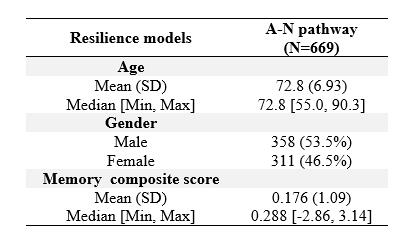
\includegraphics[scale=0.52]{Table1.jpg}
         \caption{Demographic characteristics of participants in A-N}
\end{figure}
\section{Statistical Analysis}
\subsection{Variable Selection}
Integrative factor regression model [1] was used to select potentially influential variables (regional SUVRs) to be included in the second-stage mediation analysis next step. For each modality (Amyloid and FDG), we control the confounding effects on the observed regional SURVs by regressing raw values of ROIs on the confounders including age and gender). Each two of them will be used as the exposure and mediator variables of the outcome (MEM score) in the mediation analysis. I first regress the outcome on modalities A and [N] and select regional SUVRs in these modalities that are associated with the outcome. Let $y$ be the residual of regressing MEM on confounders and $x_m$ be the vector of variables from the $m^{th}$ modality for $m=1,2.$ The considered linear regression model is $y=\sum_{m=1}^2 x'_m\beta^*_m+\epsilon$, where $\beta^*_m$ is the effects of variables from the $m^{th}$ modality, and $\epsilon$ is the error term. To account for the within- and across-modality correlations, the integrative factor model assumes that $x_m$ has a decomposition of $x_m=\Lambda_mf_m+u_m$, where $f_m$ is the vector of latent factors in the $m^{th}$ modality with their loadings as $\Lambda_m$, and $u_m$ is the idiosyncratic error. Then, Bai and Ng's methods [2] is used to estimate the number of latent factors and a principal component analysis (PCA) method to obtain the estimators of $f_m$ and $u_m$. At last, integrative factor model is implemented to regress $y$ on the estimators of $f_m$ and $u_m$ with a SCAD (smooth clipped absolute deviation) penalty to select non-zero components of $\beta^*_m$ identifying the regional SUVRs in the $m^{th}$ modality associated with the MEM. 
\begin{figure}[h]
         \centering
         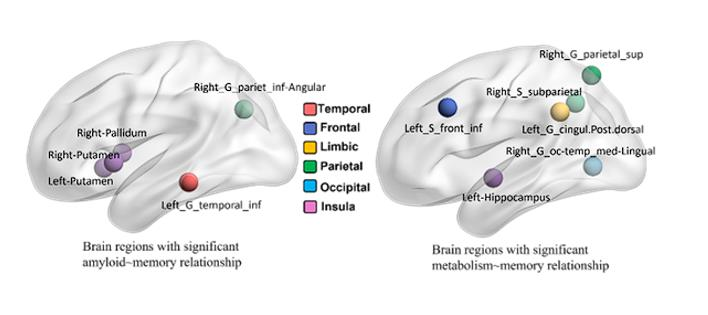
\includegraphics[scale=0.6]{Selected_Region.jpg}
         \caption{Selected brain regions from Amyloid-PET (left) and FDG-PET (right) images with respect to memory score}
\end{figure}
The final set of selected region SURVS including 5 amyloid ROIs including Amyloid.Left-G-temporal-inf, Amyloid.Right-G-pariet-inf.Angular, Amyloid.Left.Putamen, Amyloid.Right.Putamen and Amyloid.Right.Pallidum, and 6 FDG ROIs including FDG.Left-G-cingul.Post.dorsal, FDG.Left-S-front-inf, FDG.Right-G-oc.temp-med.Lingual, FDG.Right-G-parietal-sup, FDG.Right-S-subparietal and FDG.Left.Hippocampus.

\subsection{Mediation Analysis
}
After variable selection, we design the following region-to-region structural equation models (SEMs) to elucidate the mechanistic pathways between A and [N] biomarkers. In this relation, Amyloid(A) is the exposure, the independent variable. FDG([N]) is the potential mediator we want to investigate. MEM score(C) is the outcome variable. 
Three regression models are constructed to evaluate a mediation effect of the potential mediator:
\begin{equation}
    \begin{aligned}
        &\mathrm{Model}1: y=\gamma_1+\tau x_1+\epsilon_1 \\
        &\mathrm{Model}2: x_M=\gamma_2+\alpha x_1+\epsilon_2 \\
        &\mathrm{Model}3: y=\gamma_3+\tau' x_1+\beta x_M+\epsilon_3\\ 
    \end{aligned}
\end{equation}
In these models, $y$ is the dependent variable representing the outcome variable. $x_M$ is the potential mediator, FDG. $\gamma_i,i\in{1,2,3}$ are the intercept for each equation/model, while $\epsilon_i,i\in{1,2,3}$ are the error terms. $\tau$ indicates the relationship between the $x_1$, the independent variable, and $y$, the dependent variable in model 1. $\tau'$ indicates the similar relationship in model 3 adjusted for the effect of the potential mediator $x_M$. $\alpha$ represents the relationship between the independent variable and the mediator, while $\beta$ represents the relationship between the mediator and the dependent variable after controlling for the independent variable. The following two diagrams reflect the set of SEM models.
\begin{figure}[h]
         \centering
         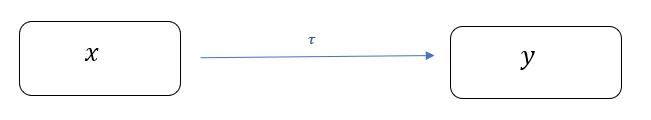
\includegraphics[scale=0.6]{diagram1.jpg}
         \caption{Relationship represented by model 1}
\end{figure}
\begin{figure}[h]
         \centering
         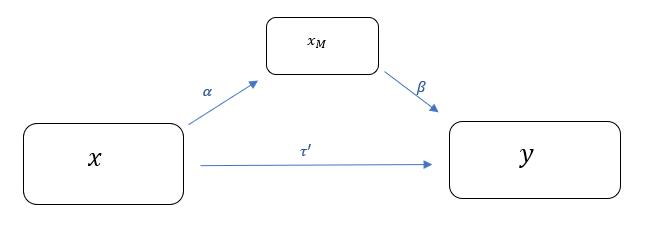
\includegraphics[scale=0.6]{diagram2.jpg}
         \caption{Relationship represented by model 2 and 3}
\end{figure}
The mediation/indirect effect is determined as $\alpha\beta=\tau-tau'$. To be more specific, $\alpha\beta$, the product of coefficients represents the amount of variance in $y$ accounted for by $x$ through the mechanism of $x_M$. The null hypothesis of Sobel test is that the indirect effect doesn’t exist, i.e.,$\alpha\beta=0$. The corresponding statistics of the Sobel test is $t=\frac{\tau-\tau'}{SE}$, where $SE=\sqrt{\alpha^2\sigma^2_{\beta}+\beta^2\sigma^2_{\alpha}}$. $\sigma^2_{\alpha}$and $\sigma^2_{\beta}$ is the variance of $\beta$ and $\alpha$ respectively. Those mediators (FDG ROIs) with significant p-value through Sobel test are believed they have mediation/indirect effect on the outcome variable. 
\begin{figure}[t]
         \centering
         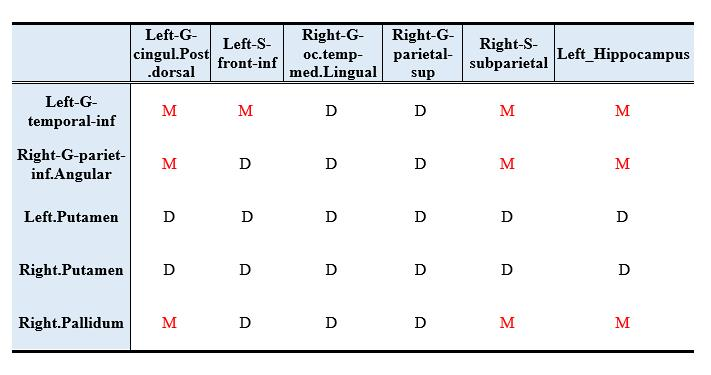
\includegraphics[scale=0.6]{Mediation_Results.jpg}
         \caption{Results of mediation analysis on relation A→N→MEM. Red and bolded "M" standards for the mediation effect of amyloid burden (A) (row) on memory decline is mediated by reduced metabolism level ([N]) (column).}
\end{figure}
As shown in table above, 10 out of 30 possible region-to-region pathways (highlighted in red) manifest a indirect effect of FDG accumulation on relation between amyloid and the decrease of memory composite score at the significance level of $p = 0.05$, where p-value is FDR-adjusted due to multiple testing problem.
\section{Conclusion}
In this project, a set of multivariate statistical inference approaches is emploed to investigate the causal relation of A and [N] biomarkers on cognitive decline adjusted for the underlying non-modifiable risk factors (as such age and APOE4 status) through high-dimensional neuroimaging phenotypes. However, this current analysis still has limitations: First, the requirement of having complete paired imaging biomarkers in the mediation analysis raises the issue of small sample size. Second, a well-classified structural equation model should be required to take the gene-by-environment interactions into account. 
\section{Reference}
[1]Li, Q. and L. Li, Integrative Factor Regression and Its Inference for Multimodal Data Analysis. Journal of the American Statistical Association, 2021: p. 1-15.\newline
[2]Bai, J. and S. Ng, Determining the Number of Factors in Approximate Factor Models. Econometrica, 2002. 70(1): p. 191-221
\end{document}
